\documentclass[12pt]{article} % use larger type; default would be 10pt
\usepackage[utf8]{inputenc} % set input encoding (not needed with XeLaTeX)

%%% PAGE DIMENSIONS
\usepackage{geometry} % to change the page dimensions
\geometry{letterpaper} % or letterpaper (US) or a5paper or....
 \geometry{margin=1in} % for example, change the margins to 2 inches all round
% \geometry{landscape} % set up the page for landscape
%   read geometry.pdf for detailed page layout information

%%% PACKAGES
\usepackage{graphicx} % support the \includegraphics command and options
\usepackage{setspace}
\doublespacing
\usepackage[parfill]{parskip} % Activate to begin paragraphs with an empty line rather than an indent
\usepackage{booktabs} % for much better looking tables
\usepackage{array} % for better arrays (eg matrices) in maths
\usepackage{paralist} % very flexible & customisable lists (eg. enumerate/itemize, etc.)
\usepackage{verbatim} % adds environment for commenting out blocks of text & for better verbatim
\usepackage{subfig} % make it possible to include more than one captioned figure/table in a single float
% These packages are all incorporated in the memoir class to one degree or another...
\usepackage{amsmath} %Allow math
\usepackage{appendix} %Allow for creation of appendicies
\usepackage{textgreek} %Allow greek text outside math mode

%Allow big first letter in Paragraph
\usepackage{type1cm}
\usepackage{lettrine}

%DEFINE VARIABLES
\newcommand{\classnumber}{AAE\:412\:-\:Team\:32:}
\newcommand{\reportnumber}{Final Project}
\newcommand{\TAname}{Dr. Gregory Blaisdell}

%%% HEADERS & FOOTERS
\usepackage{fancyhdr} % This should be set AFTER setting up the page geometry
\pagestyle{fancy} % options: empty , plain , fancy
\renewcommand{\headrulewidth}{0pt} % customise the layout...
\lhead{}\chead{}\rhead{}
\lfoot{}\cfoot{\thepage\\Purdue University}\rfoot{}

%%% SECTION TITLE APPEARANCE
\usepackage{sectsty}
\allsectionsfont{\fontsize{12}{15}\centering\textbf} % (See the fntguide.pdf for font help)
\renewcommand{\thesection}{\Roman{section}.} 
\renewcommand{\thesubsection}{\textbf{\Alph{subsection}.}}
% (This matches ConTeXt defaults)
\usepackage[font=small,labelfont=bf]{caption} % Required for specifying captions to tables and figures

\renewcommand{\appendixname}{APPENDIX} %Change  Appendix Title to spell out the word

%%% END Article customizations

%%%MATLAB CODE
\usepackage[numbered,framed]{matlab-prettifier}
\renewcommand*{\lstlistlistingname}{List of MATLAB Code Snippets} %Change MATLAB ToC Title


%%% The "real" document content comes below...

\title{\classnumber\:\reportnumber}
\author{Jay Blake\\Devin Eubanks\\Brad Lock\\Purdue University}

\begin{document}
\maketitle
\vspace{2in}
\begin{center}
    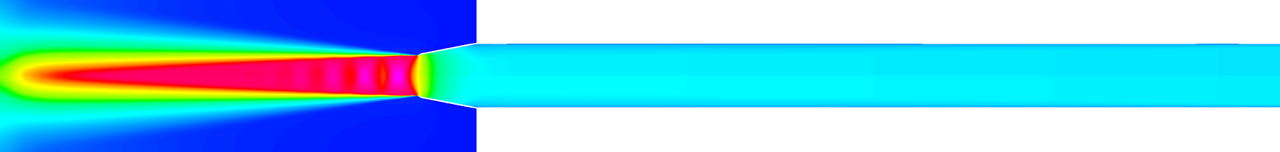
\includegraphics[width=\linewidth]{CoverPicture.png}
\end{center}
\clearpage
\begin{center}
{\Large\textbf{\classnumber\:\reportnumber}}\\
\vspace*{24pt}
Jay B. K. Blake\footnote{Engineer, School of Aeronautics and Astronautics, 701 W Stadium Ave, West Lafayette, IN 47907}, Devin M. Eubanks\footnote{Engineer, School of Aeronautics and Astronautics, 701 W Stadium Ave, West Lafayette, IN 47907}, and Bradley W. Lock\footnote{Engineer, School of Aeronautics and Astronautics, 701 W Stadium Ave, West Lafayette, IN 47907}\\
\textit{Purdue University, West Lafayette, IN, 47907}
\end{center}
\vspace*{36pt}
%Abstract
\textbf{\hspace{36pt}A Computational Fluid Dynamics simulation was ran on three nozzle geometries, defined by M. T.. Trumper, P. Behrouzi, and J. J. Mcguirk in \textit{Influence  of  nozzle  exit  conditions on  the  near-field  development  of  high  subsonic  and  underexpanded  axisymmetric  jets}. Analysis was performed on boundary layer and jet plume properties for supersonic conditions using a Nozzle Pressure Ratio of 2.2. An additional analysis was performed on one of the nozzles to determine flow properties of jet exhaust rather than air.}
\vspace*{36pt}
\section*{Nomenclature}
\begin{table}[ht]
    %\centering
    \begin{tabular}{l c l}
       $\alpha$&=&Angle of Attack\\
       CFD&=&Computational Fluid Dynamics\\
         M&=&Mach Number\\
         NPR&=&Nozzle Pressure Ratio\\
         $p$&=&Pressure\\
         $p_0$&=&Stagnation Pressure\\
         $p_a$&=&Atmospheric Pressure\\
         $\gamma$&=&Ratio of Specific Heats
    \end{tabular}
    \label{tab:nomenclature}
\end{table}
\clearpage
\section{Introduction}
\subsection{Experimental Motivation and Background}
\lettrine{A}{s} outlined in the paper by Trumper, et al., researchers set out to gain detailed knowledge of near field flow and jet plume development for different converging nozzle geometries.\cite{MilesT.Trumper2018IoNE} The goal was to use this data to reduce jet noise for civilian applications and infrared signature for military purposes. The experimental set up is shown in Figure \ref{fig:Setup}. It consisted of a high-pressure nozzle capable of air mass flow up to 0.8 kg/s at a maximum gauge pressure of 1.38 Mpa. The flow could be intercooled and dried, guaranteeing consistent flow between runs. The air was piped into the facility before passing through a 4:1 contraction into the final delivery pipe with a diameter of 75mm. This pipe could be fitted with several different test nozzles, the geometry of which will be discussed in the following subsection. In the experiment, 4 geometries were used at NPRs ranging from 1.3 to 2.4. This provided both high-subsonic and supersonic flows with the critical NPR being 1.893 for air.

\begin{center}
    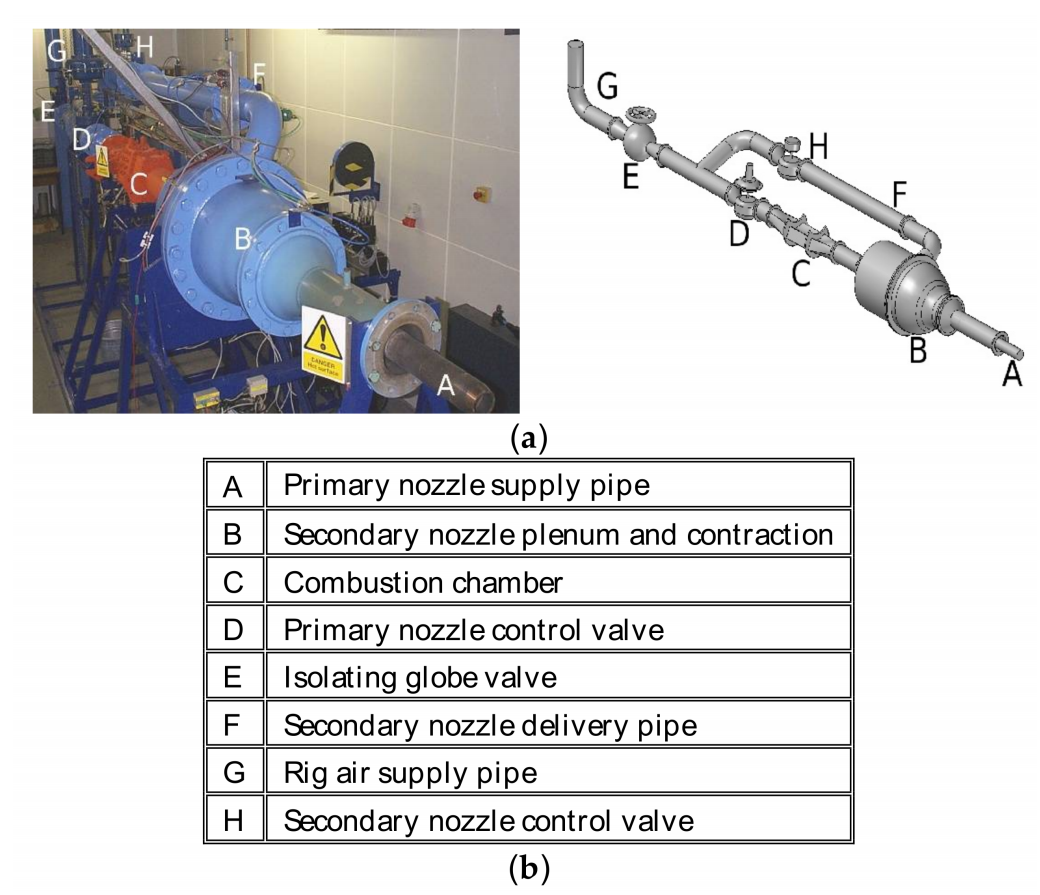
\includegraphics[width = 4in]{setup.PNG}
    \captionof{figure}{Experimental Setup\cite{MilesT.Trumper2018IoNE}}
    \label{fig:Setup}
\end{center}

\subsection{Project Motivation and Problem Definition}
The overarching motivation behind this project is to model real-world experimental results using CFD. The tests described above were used as a basis for computational modeling and used for comparison to check the validity of the model. Then, further analysis was completed and additional conclusions drawn to extend the scope of the experimental results. 

Three specific cases were chosen for CFD modeling. These cases involve running air through three of the four nozzle geometries provided at an NPR of 2.2. This NPR was chosen because it is well above the critical pressure ratio, guaranteeing that flow will reach supersonic conditions. The three nozzles used were LU48 (Nozzle (a)), LU60 (Nozzle (b)), and LU48P (Nozzle (c)) as shown in Figure \ref{fig:geometries}. Respectively, these nozzles converged to a 48mm diameter, 60mm diameter, and 48mm diameter exit. Nozzle (c) included a flat portion at the exit of length 35mm. The primary points of focus in this project are to examine the effects of nozzle diameter and parallel nozzle extension on the jet plume and flow field. 

\begin{center}
    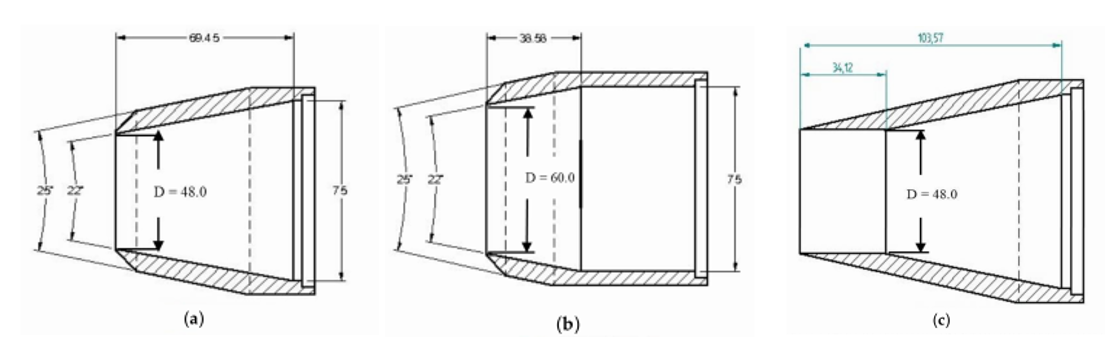
\includegraphics[width = \linewidth]{Geometries.png}
    \captionof{figure}{Geometries Modeled}
    \label{fig:geometries}
\end{center}

\section{Numerical Solution}
\subsection{Geometry}
ANSYS Fluent was used to develop a numerical solution for Nozzles (a), (b), and (c), as shown in Figure \ref{fig:geometries}. For each nozzle, Design Modeler was used to create the geometry. In the paper written by Trumper, et al., it was noted that the first 10-15 exit diameters around the output of a jet are important in the analysis of jet plumes \cite{MilesT.Trumper2018IoNE}, so the outer domain was defined out to 20 exit diameters for each case. The inlet pipe length was chosen such that the boundary layer at the nozzle inlet was 29mm, matching the boundary layer defined in the paper. The domains used are shown with meshing in Section II.B.\par

In order to determine the pipe length required to reach the proper boundary layer, the pipe was extended to 2 meters and ran in Fluent using the boundary conditions in Table \ref{tab:boundary}. Then, CFD Post was used to show the Mach contours and the location within the pipe was found visually to be 1.21 meters from the inlet, as shown in Figure \ref{fig:boundarylength}. The pipe was then shortened to this length in all geometries.

\begin{center}
    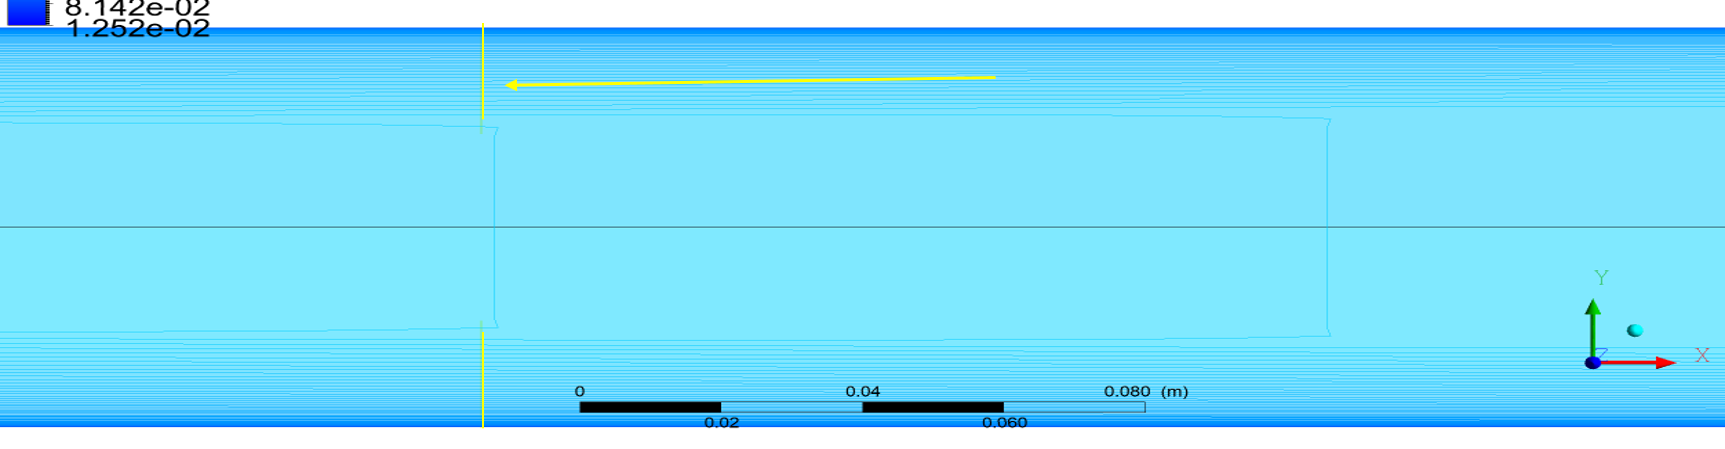
\includegraphics[width = \linewidth]{BoundaryLength.PNG}
    \captionof{figure}{CFD Post - Pipe Length}
    \label{fig:boundarylength}
\end{center}

\subsection{Meshing}\label{section:mesh}
An initial grid study was completed to create a coarse mesh to fill the geometry. The goal was set to put 10-20 cells inside the boundary layer inside the nozzle for this first mesh. To do this a roughly spaced grid was made and 1000 iterations run to gain a preliminary solution. The boundary layer was examined and the mesh refined to meet the above goal. Biasing was done to put more cells close to areas of interest\textemdash close to the nozzle walls and exit\textemdash with a gradually decreasing number of cells as the grid moves away from the areas of interest. The resulting coarse grid contains around 60,000 cells and a maximum aspect ratio of 252. A fine grid was then generated by increasing the cell divisions in each direction by a factor of two. This grid contained around 240,000 cells with a similar maximum aspect ratio of 251. An overview of the mesh for Nozzle (a) is shown in Figure \ref{fig:geomA} with a side-by-side comparison of the two meshes shown in Figure \ref{fig:gridcompareA}; the coarse grid is on the left and fine grid is on the right.

\begin{center}
    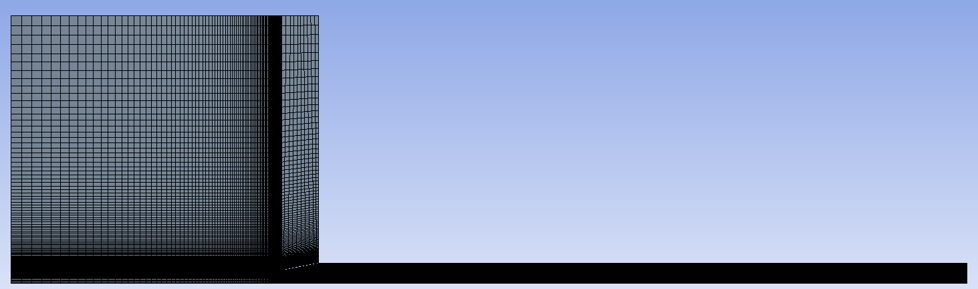
\includegraphics[width = \linewidth]{NozzleA_Mesh.PNG}
    \captionof{figure}{Nozzle (a) Coarse Mesh}
    \label{fig:geomA}
\end{center}

\begin{center}
    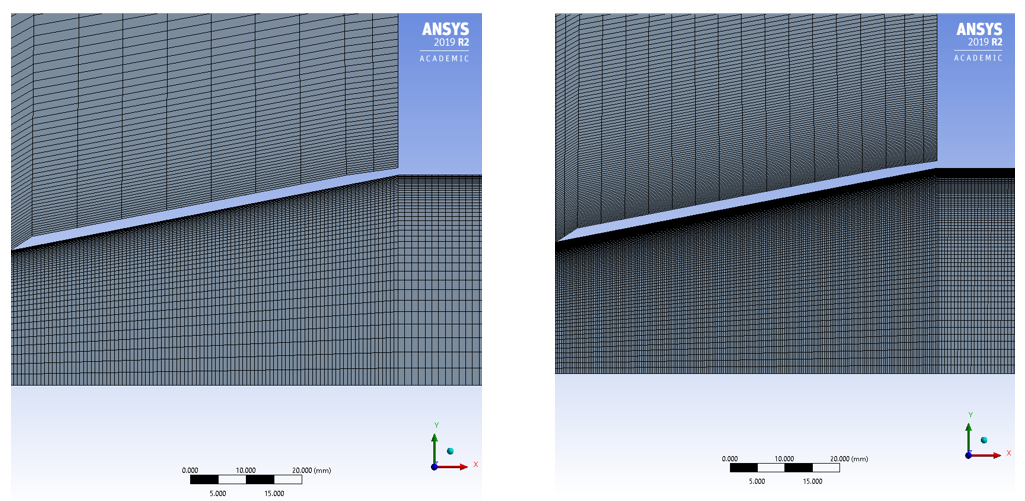
\includegraphics[width = \linewidth]{GridCompareA.png}
    \captionof{figure}{Nozzle (a) Grid Comparison}
    \label{fig:gridcompareA}
\end{center}

\clearpage

\subsection{Fluent}\label{section:fluent}
Named selections were applied to the geometries, as shown in Figure \ref{fig:namedselection}. Then, ANSYS Fluent was used to provide a CFD solution. Because the NPR used in this problem was known to create supersonic flow, a density based solver was used. Additionally, because the pipe and nozzle are round, the problem was set up with axisymmetric flow. A realizable k-\textepsilon\:model was used with a standard wall function to solve for viscosity in the flow. This model required that the fluid density be defined with an ideal gas model.

\begin{center}
    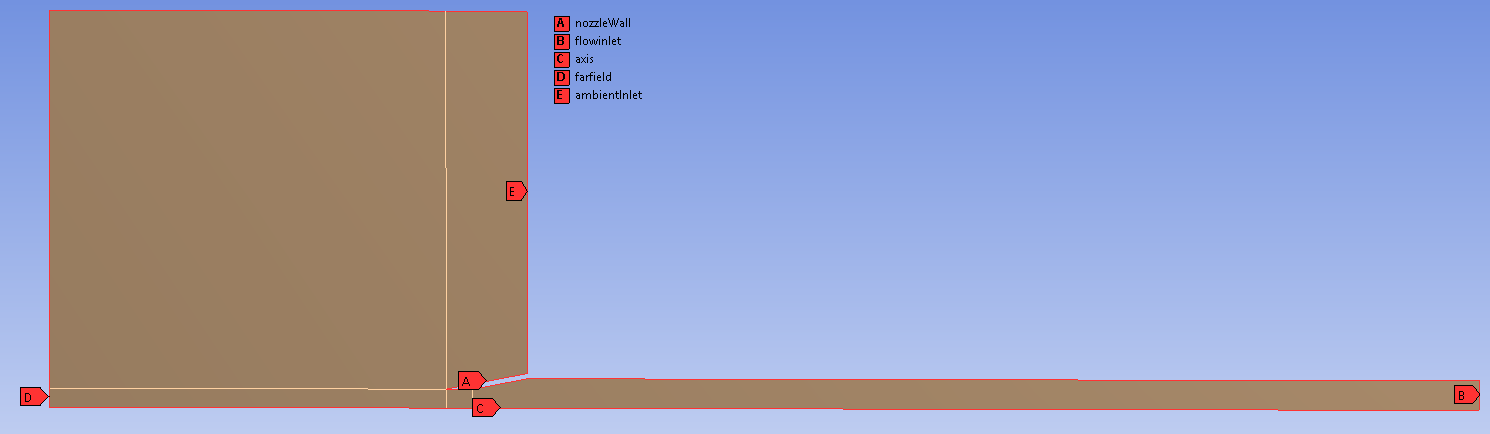
\includegraphics[width = \linewidth]{Named_Selections.PNG}
    \captionof{figure}{Named Selections}
    \label{fig:namedselection}
\end{center}

Boundary conditions, given in Table \ref{tab:boundary}, were applied to each of the named selections. The atmospheric pressure was defined as 101,325 Pa. All of the other pressures are defined as gauge pressure with respect to the atmospheric value.

\begin{table}[ht]
    \caption{Boundary Conditions}
    \centering
    \begin{tabular}{l|l}
        Named Selection&Boundary Condition\\
        \hline
        nozzleWall&wall\\
        farfield&pressure-far-field\\
        flowinlet&pressure-inlet\\
        ambientInlet&velocity-inlet\\
        axis&axis\\
        \hline
    \end{tabular}
    \label{tab:boundary}
\end{table}

Because the reference paper from Trumper, et al. used right-to-left flow, the geometry was set in ANSYS to do the same. As a result, it was required to set boundary flow velocities and Mach numbers in the negative direction. The flow inlet was defined with a gauge pressure of 121,590 Pa, matching the NPR of 2.2 as shown in Equation \ref{eq:inletpressure}.

\begin{equation}\label{eq:inletpressure}
    p_{inlet,gauge}=\left(p_{a,total}\cdot \textnormal{NPR}\right)-p_{a,total}
\end{equation}

In order to ensure the Fluent simulation would properly define flow coming out of the nozzle, a very slight fluid motion was defined for the boundary conditions outside of the nozzle. This was done using the ambient inlet and far-field. The ambient inlet was defined with an input velocity of 10 m/s in the negative-$x$ direction and a gauge pressure of 10 Pa. The far-field was defined with a Mach number of .1 in the negative-$x$ direction and a gauge pressure of 20 Pa. No additional parameters were required for the axis or wall conditions. These parameters were used for each geometry on both coarse and fine grids with an explicit formulation and a Second-Order Upwind scheme to ensure a solution that was stable and accurate. To further stabilize the solution, a Courant number of 1 was used.\par

All six cases were run using the Linux servers in the Purdue University School of Aeronautics and Astronautics CAD lab. Each case was run for a minimum of 200,000 iterations. For each case, no divergence was detected and the residuals stabilized at less than $10^{-4}$.

\section{Results}
%Begin results overview
In the assessment of simulation results, three main topics will be discussed. General comparisons will be drawn between the use of coarse and fine meshes with interpretations of $y^+$ trends, near-field flow development will be analyzed for the three varying nozzle geometries, and remarks will be made regarding the use of an alternative working fluid in the simulation.\par

\subsection{Mesh comparison}
%Begin mesh comparison
As advised by Professor Gregory Blaisdell, the scope of the team's research was to include simulations run on both coarse and fine grids. Figure \ref{fig:gridcompareA_Pressure} contains a side-by-side pressure map of the flow development for Nozzle (a) using the coarse and fine mesh. By visual inspection, it can be seen that the fine mesh renders substantially more precise and delineated shock diamonds near the exit plane as compared to the coarse mesh. Furthermore, a larger degree of precision is found in the far field flow behavior with the fine mesh where greater regions of pressure are identified. Figure \ref{fig:gridcompareA_Mach} features a similar comparison of the meshes using Mach contours instead of pressure maps. Coinciding with the observations of Figure \ref{fig:gridcompareA_Pressure}, Figure \ref{fig:gridcompareA_Mach} reveals the fine mesh having more meticulously represented shock diamonds in the near field as well as greater regions of potential core identified in the far field. Overall, the fine mesh identified certain flow behaviors not shown by the coarse mesh while providing considerably more precise results. Because of this, the remaining discussions in this publication will only focus on fine mesh results.\par

\begin{center}
    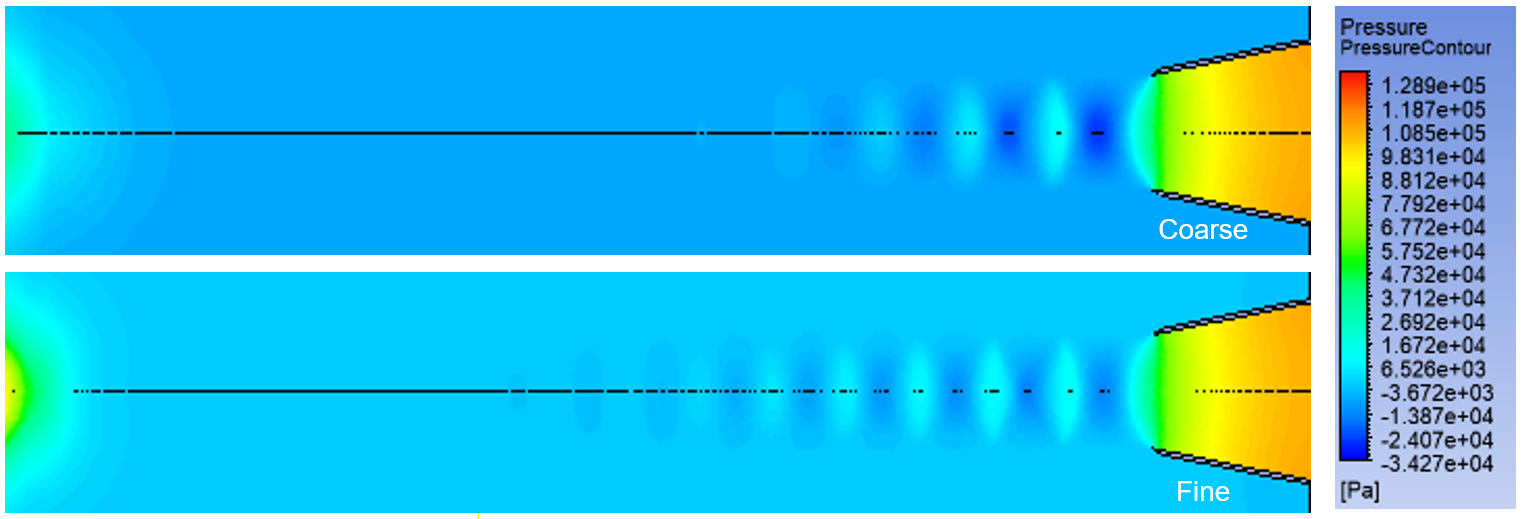
\includegraphics[width = \linewidth]{GridCompareA_Pressure.PNG}
    \captionof{figure}{Nozzle (a) Pressure Comparison}
    \label{fig:gridcompareA_Pressure}
\end{center}
\clearpage
\begin{center}
    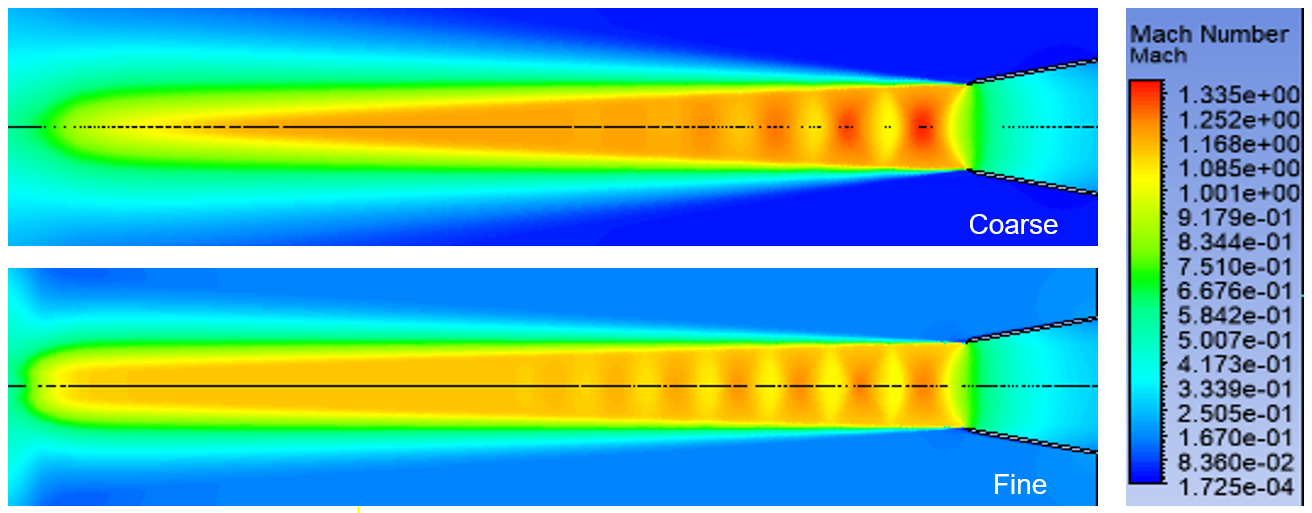
\includegraphics[width = \linewidth]{GridCompareA_Mach.PNG}
    \captionof{figure}{Nozzle (a) Mach Comparison}
    \label{fig:gridcompareA_Mach}
\end{center}

%Begin Y-Plus section:
Because the problem was set up using the k-\textepsilon\:model with standard wall functions, the desired value of $y^+$ at the nozzle wall is between 30 and 300. To reach these values, the team ensured that there were a minimum of 10 cells within the boundary layer. Graphs of the actual $y^+$ with respect to $x$ along the nozzle wall are shown for Nozzles (a), (b), and (c) in Figures \ref{fig:YPlusA}, \ref{fig:YPlusB}, and \ref{fig:YPlusC} respectively. It should be noted that the nozzle exit is at $x=0$ for all cases.

\begin{minipage}{.49\linewidth}{}
\begin{center}
    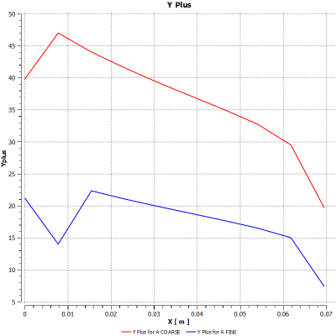
\includegraphics[width=\linewidth]{YPlus_A.png}
    \captionof{figure}{$y^+$ - Nozzle (a)}
    \label{fig:YPlusA}
\end{center}
\end{minipage}
\begin{minipage}{.49\linewidth}{}
\begin{center}
    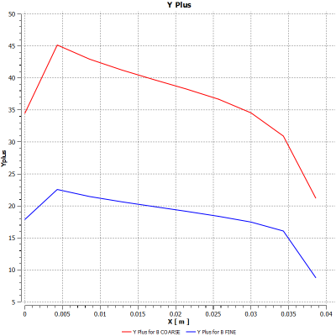
\includegraphics[width=\linewidth]{YPlus_B.png}
    \captionof{figure}{$y^+$ - Nozzle (b)}
    \label{fig:YPlusB}
\end{center}
\end{minipage}
\begin{center}
    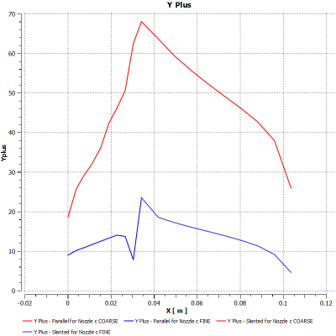
\includegraphics[width=.45\linewidth]{YPlus_C.png}
    \captionof{figure}{$y^+$ - Nozzle (c)}
    \label{fig:YPlusC}
\end{center}

It can be seen in the graphs above that the majority of the course grids met the low end of the requirements for $y^+$, but the fine grids were too fine. This fine of a grid, when combined with standard wall functions in the k-\textepsilon\:model can cause errors in boundary layer modeling. This is because the model uses the log law to estimate the boundary layer, as shown in Figure \ref{fig:loglaw}. In the figure, it can be seen that the model is accurate within the defined $y^+$ range, but loses accuracy below that. Thus, the boundary layer information in the fine grids have potential to be inaccurate.

\begin{center}
    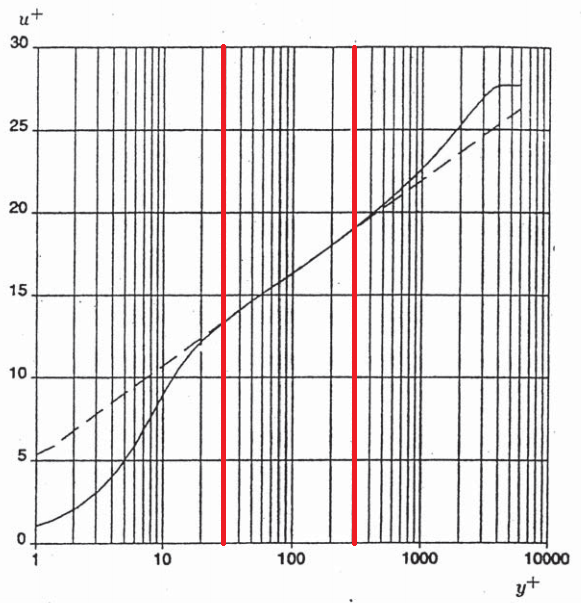
\includegraphics[width=.4\linewidth]{LogLaw.PNG}
    \captionof{figure}{The Log Law\cite{blaisdell_2019}}
    \label{fig:loglaw}
\end{center}

\subsection{Nozzle Exit Comparison}
In the comparison of the various nozzle geometries, two main factors of influence are to be discussed. The first of which being nozzle exit diameter. Nozzle (a) and Nozzle (b) share identical geometrical elements, with the exception of nozzle exit diameter; Nozzle (a) has a 48mm exit diameter and Nozzle (b) has a 60mm exit diameter. It was of the team's interest to observe the effect of exit diameter on the near-field flow development. Figure \ref{fig:NozzleComparison} contains Mach contours of the exhaust plume for all three nozzles. Visually comparing Nozzle (a) and Nozzle (b), remarkably similar trends are seen. Both nozzles have a bow shock at the nozzle exit plane, with corresponding downstream shock diamond development and quantity. One difference to note is the anticipated larger plume from Nozzle (b) which appears to reach a pressure equilibrium more rapidly than that of Nozzle (a). Despite the larger plume at the exit, it was shown that the plume in Nozzle (b) decayed faster. Much of the shock interactions in the plume are identical and align quite well.

\begin{center}
    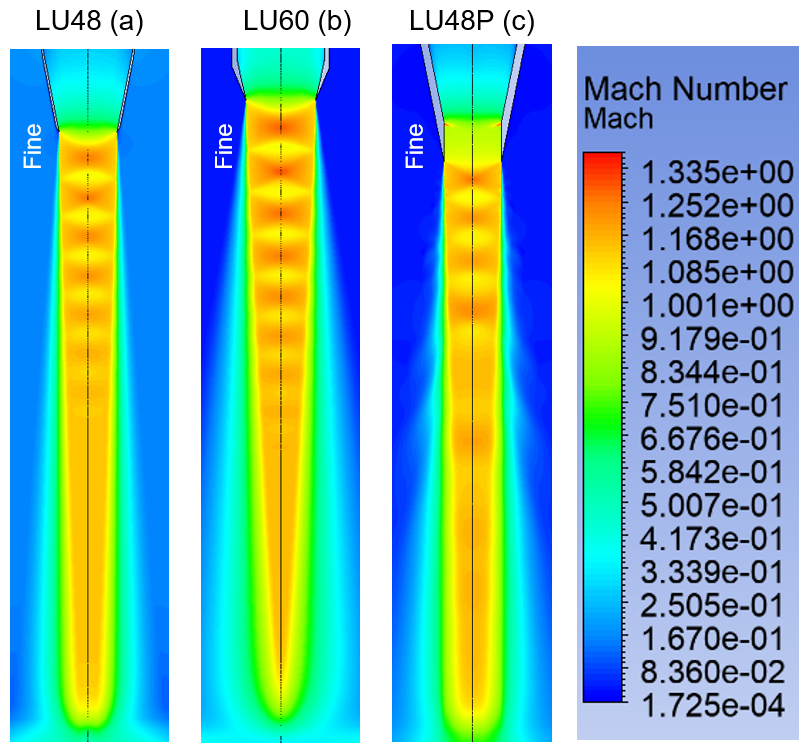
\includegraphics[width=4in]{NozzleCompare_Mach.PNG}
    \captionof{figure}{A Comparison of Nozzles (a) and (c)}
    \label{fig:NozzleComparison}
\end{center}


Shifting focus to the influence of nozzle geometry on near-field flow development, Nozzle (a) and Nozzle (c) will be compared. From the paper by Trumper, et al., which inspired these simulations and this publication, a topic of extensive discussion and concern is the Vena Contracta effect and mitigation of this phenomenon. The Vena Contracta effect\textemdash Latin for \emph{contracting vein}\textemdash is the point in a flow which has the smallest diameter\cite{mechanics_of_fluids}, and thus possesses the greatest axial velocity. This effect is of concern because it can be the source of excess jet noise, can contribute to larger infrared radar signature, and can delay the exhaust plume in reaching pressure equilibrium.\cite{MilesT.Trumper2018IoNE} Shown in Figures \ref{fig:mach_A} and \ref{fig:mach_C}, an immediately discernible difference is the flow behavior at the exit planes. Nozzle (a) demonstrates a bow shock at the exit with roughly defined shock diamonds ensuing downstream. At the same time, Nozzle (c) demonstrates Prandtl-Meyer expansion fans developing at the corners between the converging and parallel duct sections. These expansion fans later translate into a series of oblique shocks which interact with the added parallel duct section, eventually coming together to form strongly delineated shock diamonds at the exit plane. These figures are of utmost importance because they are vivid representations of the presence and absence of the Vena Contracta effect. More specifically, the red-orange region between the exit shock and first shock diamond in the plume of Nozzle (a) is precisely where the Vena Contracta effect is occurring. As illustrated in Figure \ref{fig:mach_C}, there is significantly less space between shock diamonds in the exhaust plume of Nozzle (c).

\begin{center}
    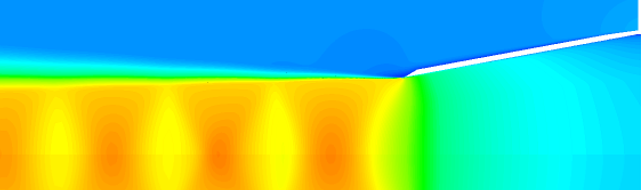
\includegraphics[width=4in]{Mach_A.png}
    \captionof{figure}{Mach Contours For Nozzle (a)}
    \label{fig:mach_A}
\end{center}

\begin{center}
    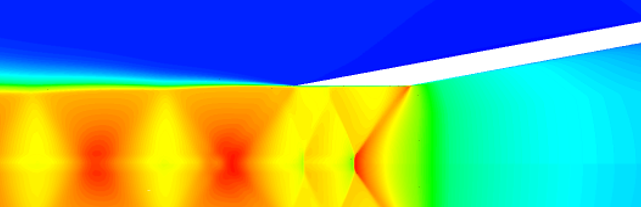
\includegraphics[width=4in]{Mach_C_Fine.png}
    \captionof{figure}{Mach Contours For Nozzle (c)}
    \label{fig:mach_C}
\end{center}

Because of the expansion that takes place within Nozzle (c), more strongly developed and flow efficient shocks are seen downstream, and thus allow no room for the Vena Contracta effect to occur. In comparison with academically validated and experimentally verified results, which are shown in Figure \ref{fig:VenaContractaReal}, the same exact phenomenon is demonstrated between both nozzles. LU48P (c) has much stronger shock interactions and less distance between shock diamonds as compared to the exhaust plume of LU48 (a).\par
Comparing the results of the CFD simulations conducted for this publication alongside the experimental results of the inspiring abstract, an appreciable degree of agreement is present. The CFD calculated comparison is shown in Figure \ref{fig:VenaContractaCFD}. Thus, as concluded in the corresponding abstract, the results of this CFD simulation suggest that the inclusion of a non-variable area addition to the nozzle minimizes the probability of the Vena Contracta effect taking place.

\begin{center}
    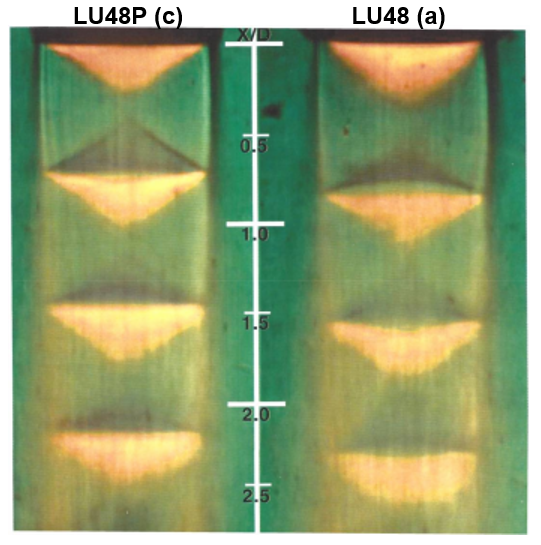
\includegraphics[width=3.5in]{VenaContracta_Real.PNG}
    \captionof{figure}{The Vena Contracta Effect (Actual) \cite{MilesT.Trumper2018IoNE}}
    \label{fig:VenaContractaReal}
\end{center}

\begin{center}
    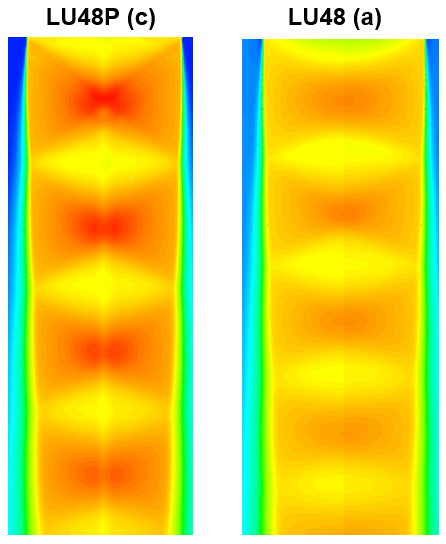
\includegraphics[width=3.5in]{VenaContracta_CFD.PNG}
    \captionof{figure}{The Vena Contracta Effect (Simulation)}
    \label{fig:VenaContractaCFD}
\end{center}


\subsection{Further Research: Jet Exhaust}

In looking for what to add to the CFD project to set it apart from the experiment, there was motivation to use a chemical approximation more comparable to jet exhaust. Table \ref{tab:pollution} shows that a substantial portion of jet exhaust is $\textnormal{CO}_2$. 

\begin{center}
    \captionof{table}{Pollution Emissions From Jet Aircraft \cite{lozano_melvin_ochheiser_1968}}
    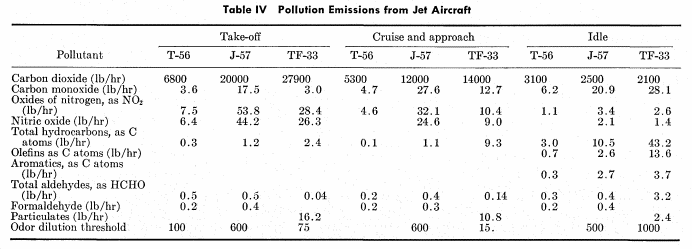
\includegraphics[width=\linewidth]{JetPollutionTable.png}
    \label{tab:pollution}
\end{center}
For this reason, it was decided that replacing the working fluid of air with $\textnormal{CO}_2$ would be a rough estimation of running a case with jet exhaust. Nozzle (a) as selected to do this run as it was the most basic geometry and could be compared the most easily. Figures \ref{fig:mach_air} and \ref{fig:mach_CO2} show the Mach contours of nozzle A using air and $\textnormal{CO}_2$ respectively.

\begin{center}
    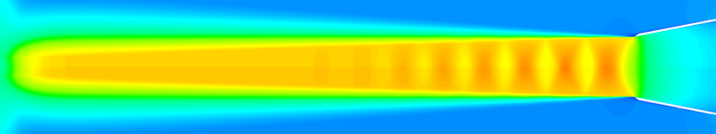
\includegraphics[width=5.5in]{Mach_Air.png}
    \captionof{figure}{Mach Contours for Air in Nozzle (a)}
    \label{fig:mach_air}
\end{center}

\begin{center}
    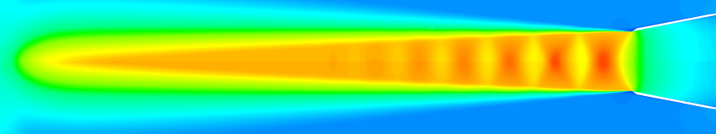
\includegraphics[width=5.5in]{Mach_CO2.png}
    \captionof{figure}{Mach Contours for Carbon Dioxide in Nozzle (a)}
    \label{fig:mach_CO2}
\end{center}

The largest observation from this case is the faster flow for $\textnormal{CO}_2$ than for air. This can be explained through the properties of the fluids. The equation for the critical NPR, the minimum pressure ratio that results in choked flow, is given in Equation \ref{eq:gammas}\cite{engineering_toolbox}.
\begin{equation}\label{eq:gammas}
\left(\dfrac{2}{\gamma+1}\right)^{\dfrac{\gamma}{\gamma-1}}
\end{equation}
Because $\gamma$ for $\textnormal{CO}_2$ is lower than that of air, the resulting critical NPR is also lower: 1.83 compared to 1.893. Given that the flow reaches sonic conditions sooner it can be reasonably concluded that for a consistent NPR\textemdash 2.2 in this case\textemdash the flow will be faster. Both contours show sonic flow in the nozzle and Mach diamonds in the near field. However, for air, they are much less defined than $\textnormal{CO}_2$’s results and decay much quicker.  One other observation made from these contours is the comparison of the plume shape extending out from the nozzle exits. While the flow is faster all around for the $\textnormal{CO}_2$, the flow profile and expansion are actually very similar to that of the air. This suggests that where plume shape is concerned, nozzle geometry is the important consideration and not the fluid being used.

Pressure contours are also included in figures \ref{fig:pressure_air} and \ref{fig:pressure_CO2} to reconfirm the observations made using the velocity. Both air and $\textnormal{CO}_2$ show alternating pockets of high and low pressure, however, the $\textnormal{CO}_2$ has much more defined and longer extending reach to this pattern. This observation is consistent with the nozzle’s Mach diamond pattern and reinforces the fact that the  $\textnormal{CO}_2$ results in a faster flow with more defined shock.

\begin{center}
    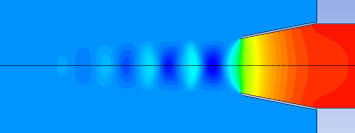
\includegraphics[width=4in]{Pressure_Air.png}
    \captionof{figure}{Pressure Contours for Air in Nozzle (a)}
    \label{fig:pressure_air}
\end{center}

\begin{center}
    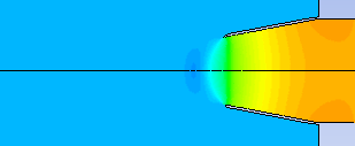
\includegraphics[width=4in]{Pressure_CO2.png}
    \captionof{figure}{Pressure Contours for Carbon Dioxide in Nozzle (a)}
    \label{fig:pressure_CO2}
\end{center}

\section{Conclusions}
\subsection{Lessons Learned}
Completing this project taught a vast amount of lessons on the topics of CFD and using ANSYS. When creating the model, it is important to pay close attention to detail. Every single parameter matters and changing just one thing can cause a lot of trouble in the solution. With that it is also common to need several different iterations to get to a valid solution. Often times, it was found that a case would be ran but not give desirable outcomes. Things would constantly need to be tweaked until a good solution, or sometimes any solution at all, was given. The idea was also reinforced that CFD is not a perfect replacement for experimental fluid dynamics. While results matched quite well to what they should, there were imperfections in some areas and in order to be 100 percent confident in results, real world tests should always be conducted. Finally, it was made clear in this project that nozzle geometry is a critical design consideration when looking at aerospace applications. A change in nozzle diameter can have a significant effect on the properties of the jet plume and a parallel nozzle exit can provide a more desired result with respect to Vena Contracta effects.

\subsection{Suggestions for Further Research}
Given more time and resources, there are several things that would ideally be explored in this project. The first addition that would be advantageous to have would be a more extensive grid study. This is based on the fact that the $y^+$ in these models dips as low as 7 in the fine grid’s case. Using k-\textepsilon, as was done in this project, the $y^+$ should ideally stay between 30 and 300. With a $y^+$ much below that there can be problems in the viscous model limiting the accuracy of the solution. Secondly, more complete analysis of the experimental scope would offer a wider range of data with which to compare. While researchers in <reference> modeled 4 different geometries and an entire range of NPRs, CFD was only done on three specific cases limiting the extent of the comparisons and reliable data. Finally, refining the jet exhaust case would be a priority moving forward. Running for more geometries and with a more accurate representation of exhaust, versus just $\textnormal{CO}_2$, could provide a much-wanted base for analysis of jet engine nozzle design.


\section{References}
%Note: Do not change this! References are added in BibTex format in AAE412Bib.bib
\nocite{*}
\begingroup
\renewcommand{\section}[2]{}%Remove Extra Title
\bibliographystyle{abbrv}
\bibliography{AAE412Bib}
\endgroup

\end{document}